\centering{\textbf{ข้อควรรู้เกี่ยวกับการเคลื่อนที่แบบฮาร์มอนิกอย่างง่าย}}
\tcblower
\begin{itemize}[leftmargin=*]
	\item[1)] 	\textbf{ขณะที่วัตถุกำลังเคลื่อนที่ผ่านจุดสมดุล (จุดตรงกลาง)}  วัตถุจะมีความเร็วสูงสุด $(v_{max})$  แต่มีความเร่ง (a)  ต่ำที่สุด \\
				\textbf{ขณะที่วัตถุอยู่ที่จุดตรงปลายของการเคลื่อนที่}  วัตถุจะมีความเร่งสูงสุด $(a_{max})$  แต่มีความเร็ว (v) ต่ำที่สุด	
	\item[2)] 	\adjustbox{valign=t}{
					\begin{minipage}{.6\linewidth}
						คาบ (T)  คือเวลาที่ใช้ในการเคลื่อนที่ครบ  1  รอบ มีหน่วยเป็นวินาที (s)\\\\
						สำหรับคาบของการเคลื่อนที่ฮาร์มอนิกอย่างง่ายแบบแกว่ง  เราสามารถหาคาบของการแกว่งได้จากสมการ
						\[ T=2\pi\sqrt{\frac{L}{g}}\]
					\end{minipage}} \hfill
				\adjustbox{valign=t}{
					\begin{minipage}{.35\linewidth}
						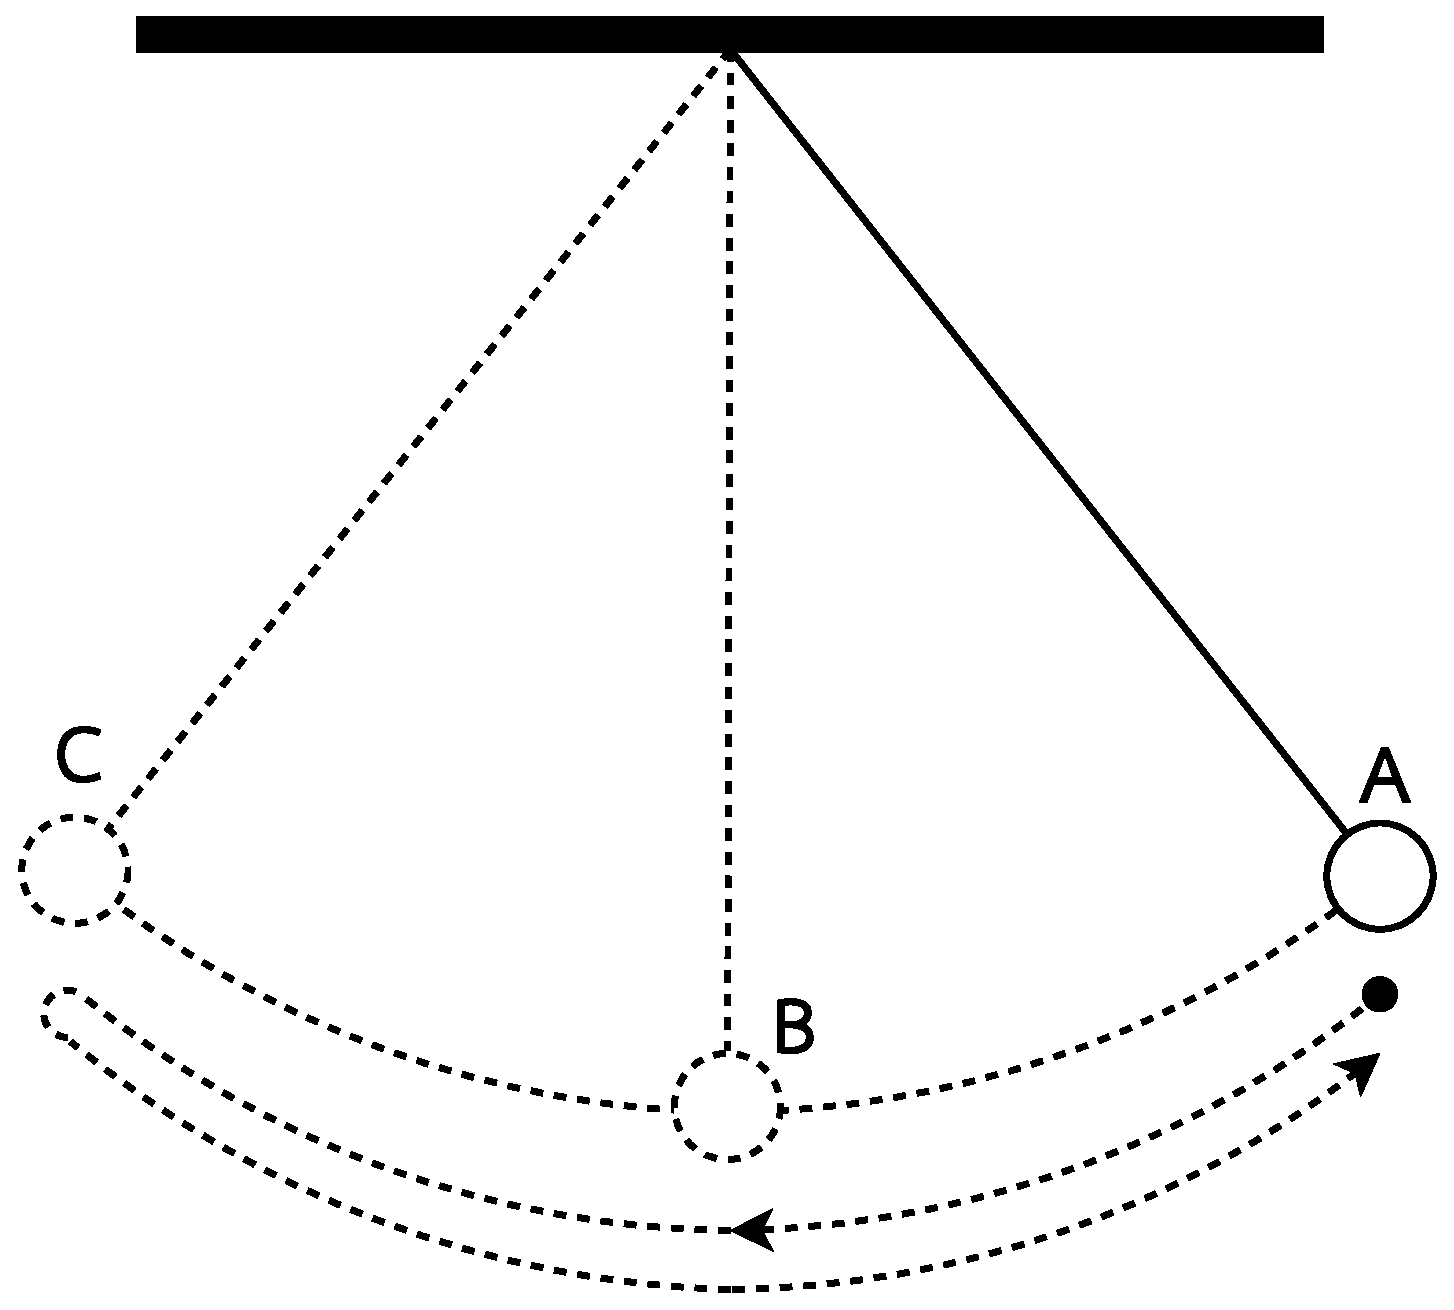
\includegraphics[width=\textwidth]{content-14.eps}
					\end{minipage}
				}
				\begin{tabbing}
					\textbf{เมื่อ} \quad 	\=T \quad 	\=\textbf{คือ} 	\=คาบของการแกว่ง  มีหน่วยเป็น วินาที (s) \\
										\>L 		\>\textbf{คือ} 	\>คือระยะจากจุดตรึงสายแกว่งถึงจุดศูนย์กลางลูกตุ้ม มีหน่วยเป็น \\
										\>			\>				\>เมตร (m)\\
										\>g			\>\textbf{คือ} 	\>คือความเร่งเนื่องจากแรงโน้มถ่วง มีหน่วยเป็น เมตร/วินาที$^2$ ($m/s^2$)
				\end{tabbing}
	\item[3)] 	ความถี่ (f)  คือจำนวนรอบที่เคลื่อนที่ได้ในหนึ่งหน่วยเวลา  มีหน่วยเป็น  รอบ/วินาที หรือเฮิรตซ์ (Hz) เราสามารถหาค่าความถี่ได้จากสมการต่อไปนี้\\
				\[ f = \frac{\text{จำนวนรอบ}}{\text{เวลา}} \qquad	\text{หรือ}	\qquad	f = \frac{1}{T}\]
				\begin{tabbing}
					\textbf{เมื่อ} \quad 	\=f \quad 	\=\textbf{คือ} 	\=ความถี่ (Hz)\\
										\>T 		\>\textbf{คือ} 	\>คาบของการเคลื่อนที่  (วินาที)
				\end{tabbing}
\end{itemize}
